%%%%%%%%%%%%%%%%%%%%%%%%%%%%%%%%%%%%%%%%%
% Daily Laboratory Book
% LaTeX Template
%
% This template has been downloaded from:
% http://www.latextemplates.com
%
% Original author:
% Frank Kuster (http://www.ctan.org/tex-archive/macros/latex/contrib/labbook/)
%
% Important note:
% This template requires the labbook.cls file to be in the same directory as the
% .tex file. The labbook.cls file provides the necessary structure to create the
% lab book.
%
% The \lipsum[#] commands throughout this template generate dummy text
% to fill the template out. These commands should all be removed when 
% writing lab book content.
%
% HOW TO USE THIS TEMPLATE 
% Each day in the lab consists of three main things:
%
% 1. LABDAY: The first thing to put is the \labday{} command with a date in 
% curly brackets, this will make a new page and put the date in big letters 
% at the top.
%
% 2. EXPERIMENT: Next you need to specify what experiment(s) you are 
% working on with an \experiment{} command with the experiment shorthand 
% in the curly brackets. The experiment shorthand is defined in the 
% 'DEFINITION OF EXPERIMENTS' section below, this means you can 
% say \experiment{pcr} and the actual text written to the PDF will be what 
% you set the 'pcr' experiment to be. If the experiment is a one off, you can 
% just write it in the bracket without creating a shorthand. Note: if you don't 
% want to have an experiment, just leave this out and it won't be printed.
%
% 3. CONTENT: Following the experiment is the content, i.e. what progress 
% you made on the experiment that day.
%
%%%%%%%%%%%%%%%%%%%%%%%%%%%%%%%%%%%%%%%%%

%----------------------------------------------------------------------------------------
%	PACKAGES AND OTHER DOCUMENT CONFIGURATIONS
%----------------------------------------------------------------------------------------

\documentclass[idxtotoc,hyperref,openany]{labbook} % 'openany' here removes the gap page between days, erase it to restore this gap; 'oneside' can also be added to remove the shift that odd pages have to the right for easier reading

\def\bA{\mbox{\boldmath$ A$}}
\def\bB{\mbox{\boldmath$ B$}}
\def\bC{\mbox{\boldmath$ C$}}
\def\bD{\mbox{\boldmath$ D$}}
\def\bE{\mbox{\boldmath$ E$}}
\def\bF{\mbox{\boldmath$ F$}}
\def\bG{\mbox{\boldmath$ G$}}
\def\bH{\mbox{\boldmath$ H$}}
\def\bI{\mbox{\boldmath$ I$}}
\def\bJ{\mbox{\boldmath$ J$}}
\def\bK{\mbox{\boldmath$ K$}}
\def\bL{\mbox{\boldmath$ L$}}
\def\bM{\mbox{\boldmath$ M$}}
\def\bN{\mbox{\boldmath$ N$}}
\def\bO{\mbox{\boldmath$ O$}}
\def\bP{\mbox{\boldmath$ P$}}
\def\bQ{\mbox{\boldmath$ Q$}}
\def\bR{\mbox{\boldmath$ R$}}
\def\bS{\mbox{\boldmath$ S$}}
\def\bT{\mbox{\boldmath$ T$}}
\def\bU{\mbox{\boldmath$ U$}}
\def\bV{\mbox{\boldmath$ V$}}
\def\bW{\mbox{\boldmath$ W$}}
\def\bX{\mbox{\boldmath$ X$}}
\def\bY{\mbox{\boldmath$ Y$}}
\def\bZ{\mbox{\boldmath$ Z$}}
\def\ba{\mbox{\boldmath$ a$}}
\def\bb{\mbox{\boldmath$ b$}}
\def\bc{\mbox{\boldmath$ c$}}
\def\bd{\mbox{\boldmath$ d$}}
\def\be{\mbox{\boldmath$ e$}}
\def\bff{\mbox{\boldmath$ f$}}
\def\bg{\mbox{\boldmath$ g$}}
\def\bh{\mbox{\boldmath$ h$}}
\def\bi{\mbox{\boldmath$ i$}}
\def\bj{\mbox{\boldmath$ j$}}
\def\bk{\mbox{\boldmath$ k$}}
\def\bl{\mbox{\boldmath$ l$}}
\def\bm{\mbox{\boldmath$ m$}}
\def\bn{\mbox{\boldmath$ n$}}
\def\bo{\mbox{\boldmath$ o$}}
\def\bp{\mbox{\boldmath$ p$}}
\def\bq{\mbox{\boldmath$ q$}}
\def\br{\mbox{\boldmath$ r$}}
\def\bs{\mbox{\boldmath$ s$}}
\def\bt{\mbox{\boldmath$ t$}}
\def\bu{\mbox{\boldmath$ u$}}
\def\bv{\mbox{\boldmath$ v$}}
\def\bw{\mbox{\boldmath$ w$}}
\def\bx{\mbox{\boldmath$ x$}}
\def\by{\mbox{\boldmath$ y$}}
\def\bz{\mbox{\boldmath$ z$}}


\usepackage[ 
  backref=page,
  pdfpagelabels=true,
  plainpages=false,
  colorlinks=true,
  bookmarks=true,
  pdfview=FitB]{hyperref} % Required for the hyperlinks within the PDF
  
  \usepackage{graphicx}
  
  \usepackage{amsmath}
  \usepackage{bm}
%  \usepackage{bbm}
  %\usepackage{mathrsfs}
  \usepackage{subcaption}
  \usepackage{epsfig}
  \usepackage{amsfonts}
  \usepackage{amssymb}
  \usepackage{wrapfig}
  \usepackage{psfrag}
  \usepackage{hyperref}
%  \usepackage[ruled,commentsnumbered]{algorithm2e}

\usepackage{listings}
\usepackage{color}

\definecolor{dkgreen}{rgb}{0,0.6,0}
\definecolor{gray}{rgb}{0.5,0.5,0.5}
\definecolor{mauve}{rgb}{0.58,0,0.82}

\lstset{frame=tb,
	language=Java,
	aboveskip=3mm,
	belowskip=3mm,
	showstringspaces=false,
	columns=flexible,
	basicstyle={\small\ttfamily},
	numbers=none,
	numberstyle=\tiny\color{gray},
	keywordstyle=\color{blue},
	commentstyle=\color{dkgreen},
	stringstyle=\color{mauve},
	breaklines=true,
	breakatwhitespace=true,
	tabsize=3
}
  
\usepackage{booktabs} % Required for the top and bottom rules in the table
\usepackage{float} % Required for specifying the exact location of a figure or table
\usepackage{graphicx} % Required for including images
\usepackage{lipsum} % Used for inserting dummy 'Lorem ipsum' text into the template

\newcommand{\HRule}{\rule{\linewidth}{0.5mm}} % Command to make the lines in the title page
\setlength\parindent{0pt} % Removes all indentation from paragraphs

%----------------------------------------------------------------------------------------
%	DEFINITION OF EXPERIMENTS
%----------------------------------------------------------------------------------------

\newexperiment{example}{A mathematical derivation of the free energy considering adhesion}
\newexperiment{example2}{deal.ii Code snippet of the free energy formulation}
\newexperiment{example3}{Phase field simulations results with adhesion term}
\newexperiment{example4}{Equivalence of Shape and Material Model}
\newexperiment{example5}{Equivalent Model Results using MATLAB}
%\newexperiment{shorthand}{Description of the experiment}

%---------------------------------------------------------------------------------------

\begin{document}

%----------------------------------------------------------------------------------------
%	TITLE PAGE
%----------------------------------------------------------------------------------------

\frontmatter % Use Roman numerals for page numbers
\title{
\begin{center}
\HRule \\[0.4cm]
{\Huge \bfseries Computational Mechanics and Multi-Physics \\[0.5cm] \Large Doctor of Philosophy}\\[0.4cm] % Degree
\HRule \\[1.5cm]
\end{center}
}
\author{\Huge Debabrata Auddya \\ \\ \LARGE auddya@wisc.edu \\[2cm]} % Your name and email address
\date{Beginning 6th June 2018} % Beginning date

\maketitle

\tableofcontents

\mainmatter % Use Arabic numerals for page numbers

%----------------------------------------------------------------------------------------
%	LAB BOOK CONTENTS
%----------------------------------------------------------------------------------------

% Blank template to use for new days:

%\labday{Day, Date Month Year}

%\experiment{}

%Text

%-----------------------------------------

%\experiment{}

%Text

%----------------------------------------------------------------------------------------

\labday{Wednesday, 6 June 2018}

\experiment{example}

\section{A phase field formulation for cell growth, division and contact considering cell adhesion}

Uptil previous literature, and extensive study has been perfomed to model a phase field representation of scalar fields. Several terms are considered for this treatment such as phase segregation of cell interior from the extra cellular matrix, intercellular repulsion (by penalising overlapping scalar field) and also considering certain boundary conditions which confine the cell evolution within a certain boundary. In this formulation we are going to consider adhesion between cells which essentially play a key role in soft packing. 

\section{Mathematical analysis of the revised model}
Let $\Omega\in \mathbb{R}^2$ with a smooth boundary $\partial \Omega$. Scalar fields $c_k, \;k = 1,\dots,N$ with $c_k \in [0,1]$ serve to delineate the interior and exterior of the cell numbered $k$. Here, the interior of cell $k$ is $\omega_k \subset \Omega$, where $\omega_k = \{ \bX \in \Omega\vert c_k(\bX) =1\}$. The exterior is $\Omega\backslash\omega_k$. The free energy density function is built up beginning with the following form:
\begin{equation}
\psi_1(c_k) = \alpha c_k^2(c_k-1)^2 + \frac{\kappa}{2}\vert\nabla c_k\vert^2 
\label{equ:psi1}
\end{equation}
where the double-well term, $f(c_k) = \alpha c_k^2(c_k-1)^2$, enforces segregation into $\omega_k$ and $\Omega\backslash\omega_k$. In Equation \eqref{equ:psi1}, the second term enforces a diffuse cell-matrix interface (the cell membrane) of finite thickness, where $\kappa$ controls the interface thickness, and thereby the interfacial energy. For $N$ cells in $\Omega$, the above free energy density needs to be extended to model contact by adding a cell-cell repulsion term. The total free energy of the multi-cell aggregate is a functional $\Pi[\bc]$, defined as
\begin{align}
\Pi[\bc] &:= \int\limits_\Omega \psi(\bc,\nabla c) ~\text{d}V\nonumber\\
&=\int\limits_\Omega \left(\sum_{k=1}^{N} f(c_k) + \sum_{k=1}^{N} \frac{\kappa}{2}\vert\nabla c_k\vert^2 + \sum_{l\ne k}\sum_{k=1}^{N}\lambda c_k^2 c_l^2 + \sum_{l\ne k}\sum_{k=1}^{N}\gamma\nabla c_k \nabla c_l \right) ~\text{d}V.
\label{equ:energy}
\end{align}

Here, $\bc = \{c_1,\dots,c_N\}$,$\lambda$ is a penalty coefficient that enforces repulsion and $\gamma$ is another penalty coefficient that enforces adhesion between any two cells $k,l$ thus modelling cell contact.

Taking the variational derivative with respect to $c_k$ in Equation \eqref{equ:energy} yields

\begin{align}
\delta \Pi_k[\bc;w] =  & \left.\frac{\text{d}}{\text{d}\epsilon} \int\limits_{\Omega} \sum_{k=1}^{N} \left(f(c_k+\epsilon w) + \frac{\kappa}{2}\vert\nabla (c_k+\epsilon w)\vert^2+ \sum_{l\ne k}\lambda (c_k+\epsilon w)^2 c_l^2 + \sum_{l\ne k}\gamma \nabla(c_k+\epsilon w) \nabla c_l \right)  ~\text{d}V \right|_{\epsilon=0} \nonumber\\
=&\int\limits_{\Omega} \left(w f^\prime(c_k) - w \kappa \Delta  c_k  + w \sum_{l\ne k}2\lambda  c_k c_l^2 - \sum_{l\ne k}\gamma\nabla w \nabla c_l \right) ~dV + \int\limits_{\partial \Omega}   w \kappa \nabla c_k \cdot \bn dS \nonumber\\
=&\int\limits_{\Omega} w \left( f^\prime(c_k) -  \kappa \Delta  c_k  +  \sum_{l\ne k}2\lambda  c_k c_l^2 - \sum_{l\ne k}\gamma\nabla^{2} c_l \right) ~dV + \int\limits_{\partial \Omega}   w \kappa \nabla c_k \cdot \bn   ~dS
\end{align} 

where $\bn$ is the unit outward normal vector to $\partial \Omega$. The chemical potential of the $k^\text{th}$ cell is identified as, 

\begin{equation}
\mu_k  = f^\prime(c_k) -  \kappa \Delta c_k + \sum_{l\ne k}2\lambda  c_k c_l^2 - \sum_{l\ne k}\gamma\nabla^{2} c_l 
\label{equ:chemo_potential}
\end{equation}

At equilibrium, $\delta_k \Pi[\bc;w] =0$ for the $k^\text{th}$ cell, yielding $\mu_k = 0$ in $\Omega$, and $\kappa \nabla c_k \cdot \bn = 0$ on $\partial \Omega$. 

The following parabolic partial differential equation, popularly known as the Cahn-Hilliard equation \cite{Cahn1958}, imposes the conserved dynamics that governs the delineation and growth of the $N-$cell agglomerate, and of repulsion between cell pairs:
\begin{equation}
\frac{\partial c_k}{\partial t} = -~\nabla \cdot (-M\nabla \mu_k) + s_k
\label{equ:dynamic}
\end{equation}
where the source term $s_k$ has been introduced, and $M$ is the mobility, assumed to be constant. The dynamics of the multi-cell soft packing problem is governed by Equation \eqref{equ:dynamic} with the thermodynamics prescribed by Equation \eqref{equ:chemo_potential} and boundary conditions $\kappa \nabla c_k \cdot \bn = 0$, $c_k=0$ on $\partial\Omega$ for $k = 1,\dots N$.

%-----------------------------------------

\labday{Tuesday, 12th June 2018}

\experiment{example2} % Multiple experiments can be included in a single day, this allows you to segment what was done each day into separate categories

The code is modified to include the adhesion term in the free energy formulation.Observe here that the change is incorporated in the chemical potential residual term and the corresponding penalty term is included along with an optimised value of the gamma which controls the phenomenon between two cells. Later we will present different values of gamma for which the phase field simulation showed observable results. 


\begin{lstlisting}
else if(ck==1){
Sacado::Fad::DFad<double> dfdc  = dFdC;
//add cross penalty terms to free energy
for (unsigned int cDof2=0; cDof2<CDOFs; cDof2++){
if (cDof2!=cDof) dfdc += 200*c[cDof][q]*c[cDof2][q]*c[cDof2][q];
}
//add surface buffer zone
if (cell->at_boundary()){
dfdc += 200*c[cDof][q]*1.0*1.0;
}
//
R[i] +=  fe_values.shape_value(i, q)*(mu[cDof][q] - dfdc)*fe_values.JxW(q);
//R[i] +=  fe_values.shape_value(i, q)*(mu[q] - dfdc - defMap.W[q] - pressure*defMap.divU[q])*fe_values.JxW(q);
for (unsigned int j = 0; j < dim; j++){
Sacado::Fad::DFad<double> Kjj= Kappa[j];
Sacado::Fad::DFad<double> kc_j= c_j[cDof][q][j]*Kjj; // Kjj*C_j
R[i] -= fe_values.shape_grad(i, q)[j]*(kc_j)*fe_values.JxW(q);
for (unsigned int cDof2=0; cDof2<CDOFs; cDof2++){
if (cDof2!=cDof){
R[i] -=  0.00085*fe_values.shape_grad(i,q)[j]*c_j[cDof2][q][j]*fe_values.JxW(q);
}
}
}
\end{lstlisting}

%-----------------------------------------

\labday{Wednesday, 13th June 2018}

\experiment{example3}

We present the phase field simulation results here considering the adhesion term and varying admissible values of gamma and the order parameters. All the images are captured at 150th iteration of the problem.  

\begin{figure}[h!]
	\centering
	\begin{subfigure}[h!]{0.4\textwidth}
		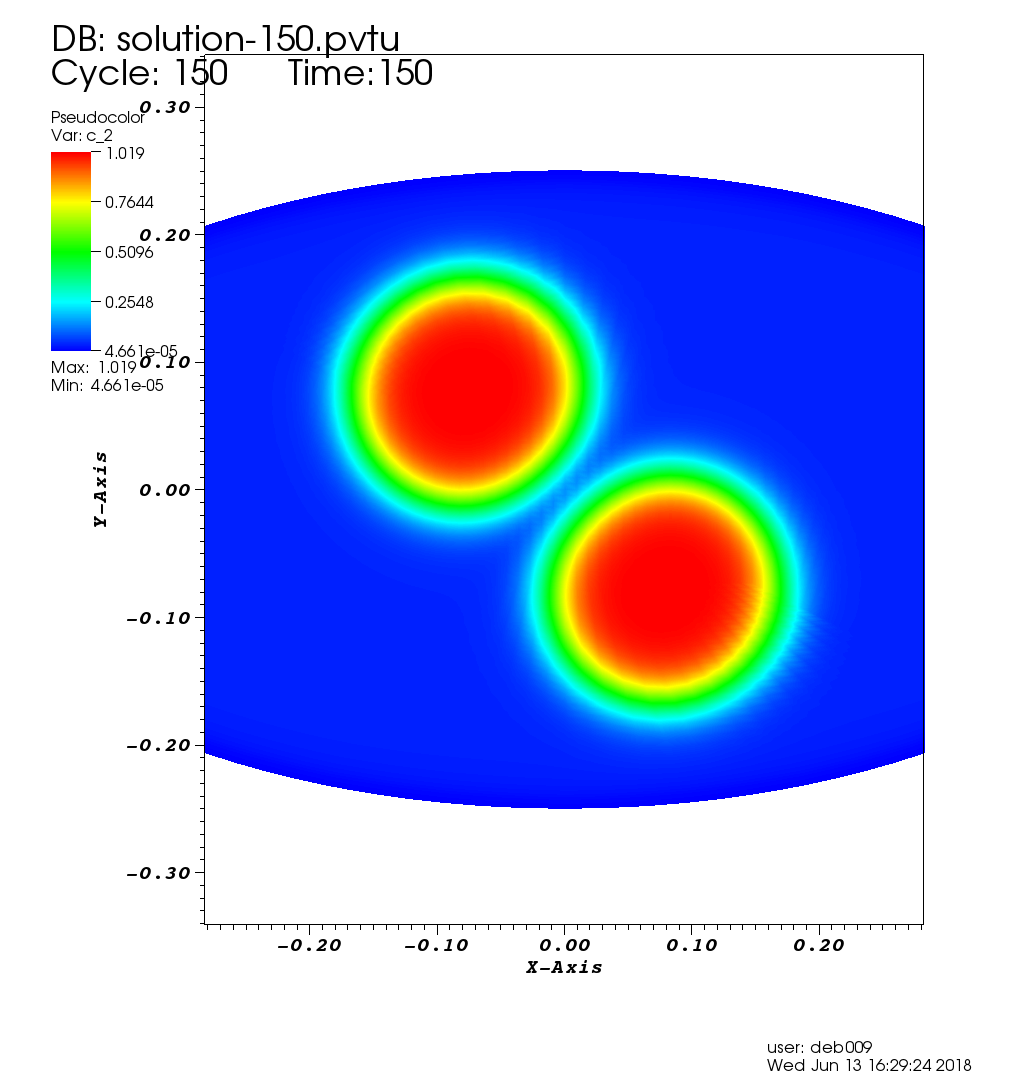
\includegraphics[width=\textwidth]{0.png}
		\caption{For $\gamma$ = 0.0}
		\label{fig:0.png}
	\end{subfigure}
	\begin{subfigure}[h!]{0.4\textwidth}
		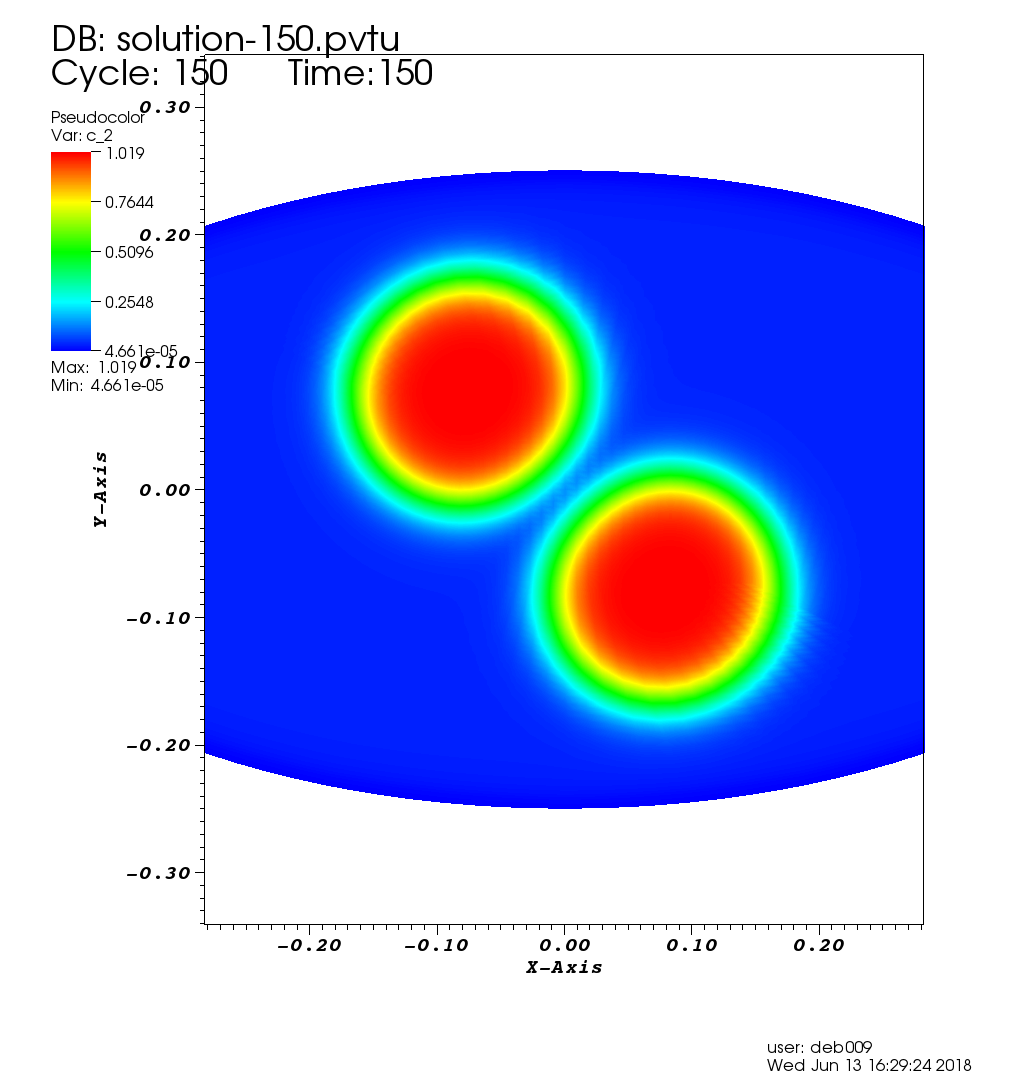
\includegraphics[width=\textwidth]{1e_05.png}
		\caption{For $\gamma$ = 1e-05}
		\label{fig:1e_05.png}
	\end{subfigure}
	\begin{subfigure}[h!]{0.4\textwidth}
		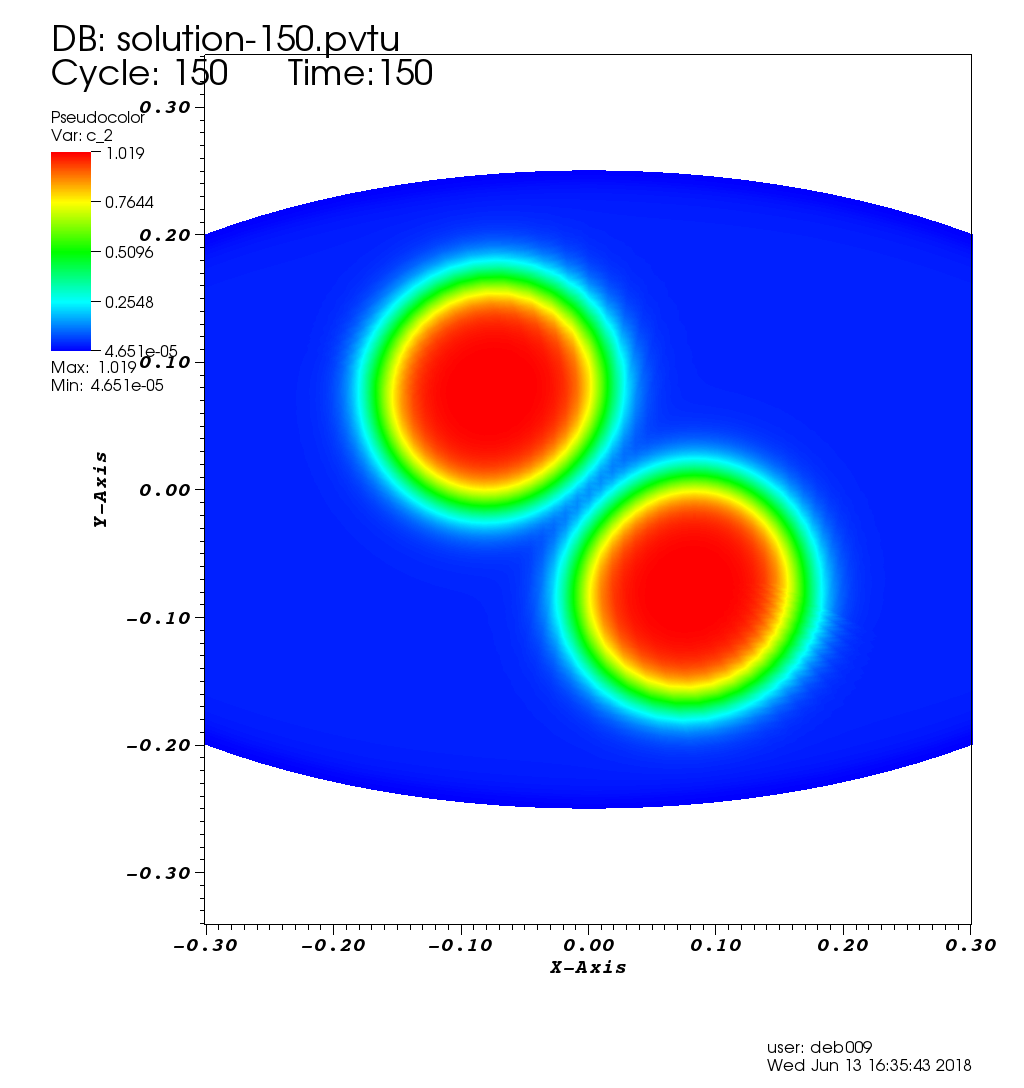
\includegraphics[width=\textwidth]{1e_06.png}
		\caption{For $\gamma$ = 1e-06}
		\label{fig:1e_06.png}
	\end{subfigure}
	\begin{subfigure}[h!]{0.4\textwidth}
		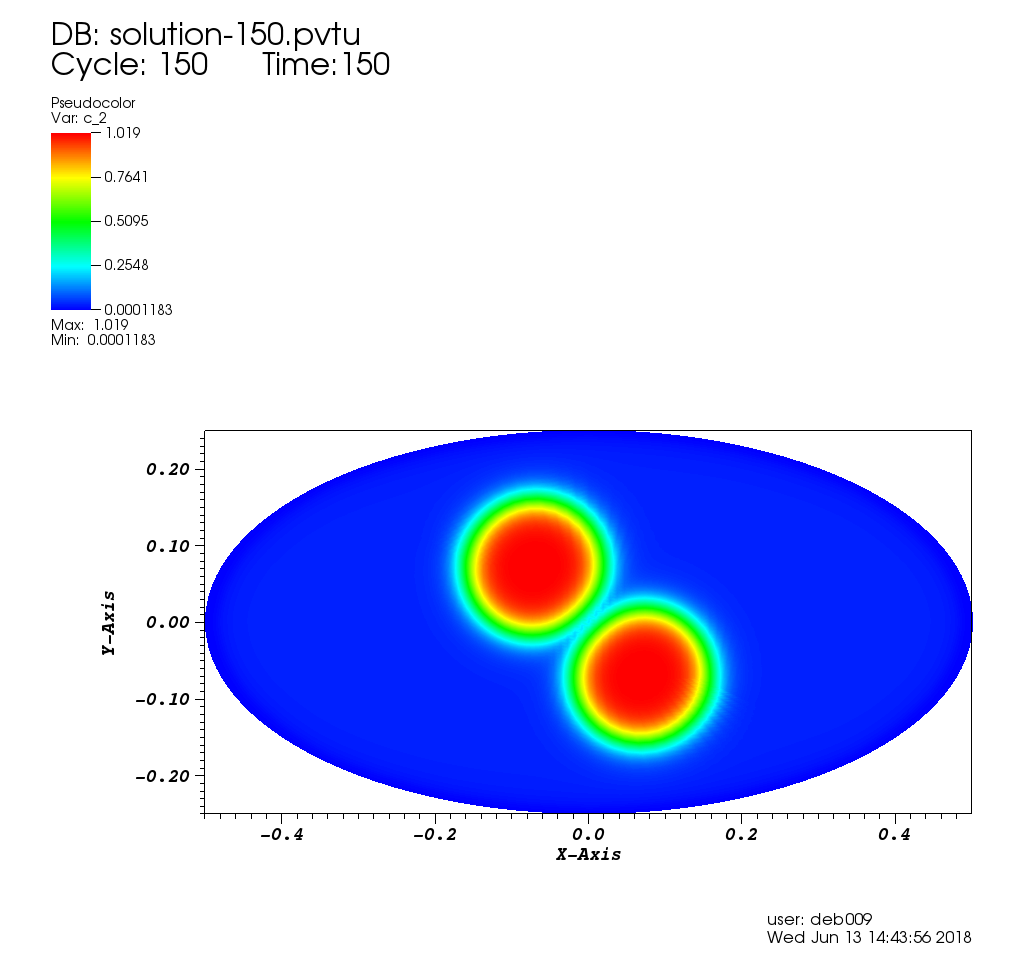
\includegraphics[width=\textwidth]{4e_04.png}
		\caption{For $\gamma$ = 4e-04}
		\label{fig:4e_04.png}
	\end{subfigure}
    \begin{subfigure}[h!]{0.4\textwidth}
    	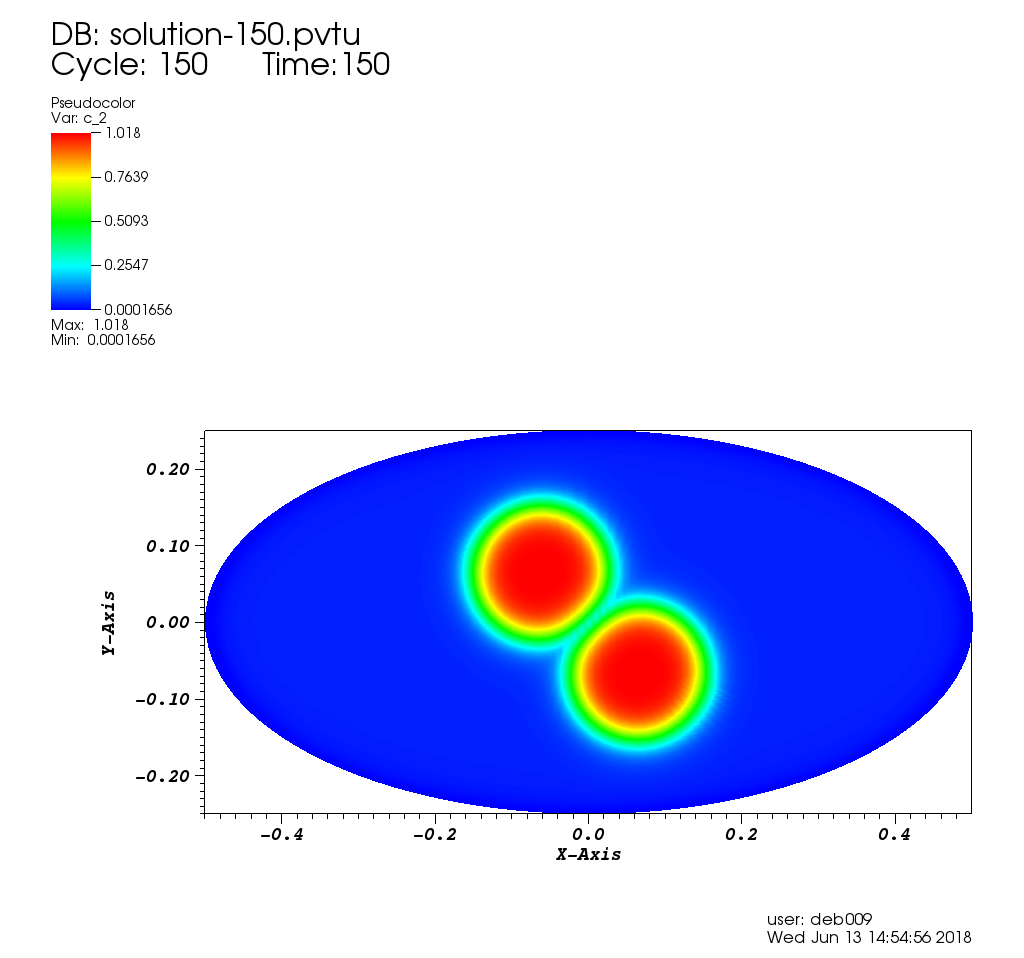
\includegraphics[width=\textwidth]{6e_04.png}
    	\caption{For $\gamma$ = 6e-04}
    	\label{fig:6e_04.png}
    \end{subfigure}
    \begin{subfigure}[h!]{0.4\textwidth}
    	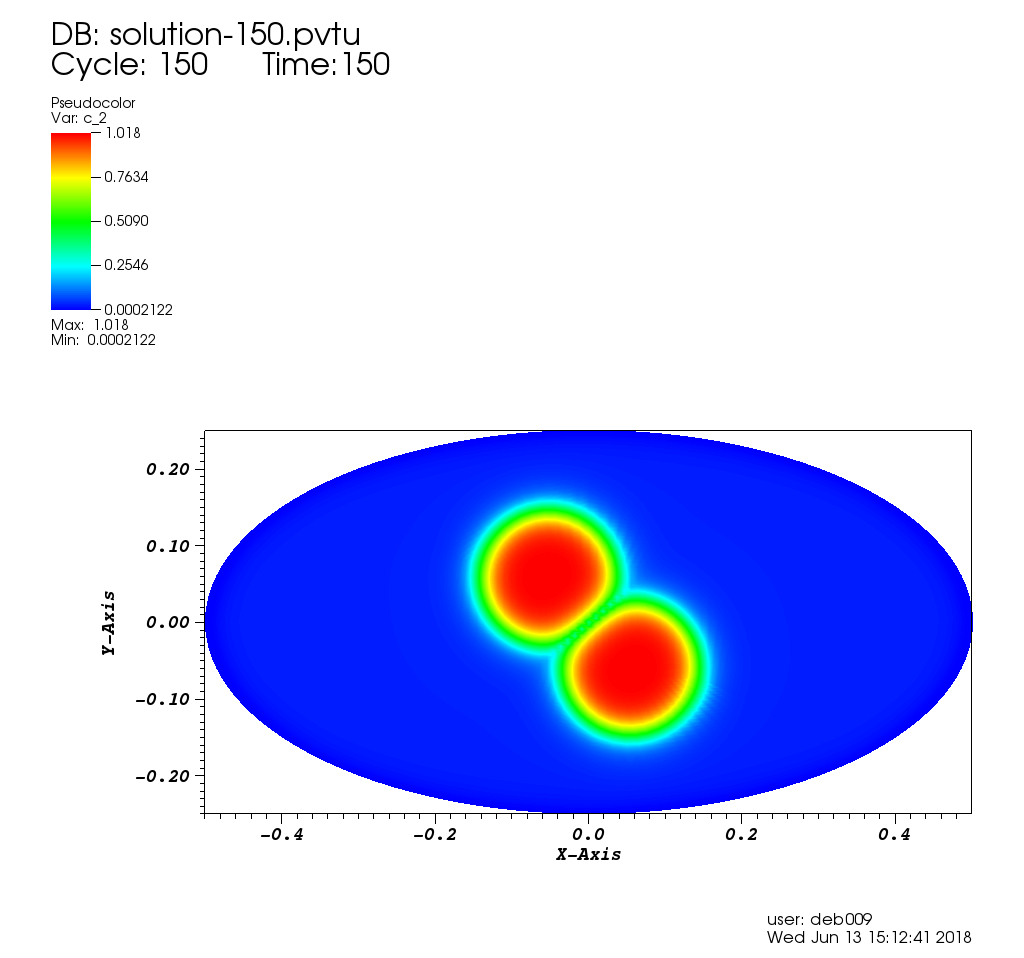
\includegraphics[width=\textwidth]{8e_04.png}
    	\caption{For $\gamma$ = 8e-04}
    	\label{fig:8e_04.png}
    \end{subfigure}
	\caption\Large\textbf{A demonstration of adhesion for different values of $\gamma$.}
\end{figure}
%----------------------------------------------------------------------------------------

\labday{Tuesday, 26th June 2018}

\experiment{example4}

%\begin{table}[H]
%\begin{tabular}{l l l}
%\toprule
%\textbf{Groups} & \textbf{Treatment X} & \textbf{Treatment Y} \\
%\toprule
%1 & 0.2 & 0.8\\
%2 & 0.17 & 0.7\\
%3 & 0.24 & 0.75\\
%4 & 0.68 & 0.3\\
%\bottomrule
%\end{tabular}
%\caption{The effects of treatments X and Y on the four groups studied.}
%\label{tab:treatments_xy}
%\end{table}
%
%Table \ref{tab:treatments_xy} shows that groups 1-3 reacted similarly to the two treatments but group 4 showed a reversed reaction.

We present here a comparison between the shape model of the cell-packing formulation (essentially soft packing) and the Mooney-Rivlin material model. We present here a mathematical equivalence of the shape and material model for this soft packing problem to illustrate an empirical relationship between them. 

\section{The Shape Model}
\begin{align}
\Pi_s = & \sum_i \delta_i (I_i - I_i^{Ref}) \nonumber\\
=& \delta_1 (I_1 - I_1^{Ref})^2 + \delta_2 (I_2 - I_2^{Ref})^2 \nonumber\\
=& \delta_1 (\frac{\pi}{4}nR(\frac{R}{2})^3 - \frac{\pi R^4}{4}) + \delta_2 (\frac{\pi}{4}(nR)^3(\frac{R}{2}) - \frac{\pi R^4}{4})\nonumber\\
=& (\frac{\pi R^4}{4})^2(\delta_1 (\frac{1}{n^2}-1)^2 + \delta_2(n^2 - 1)^2)
\end{align}

The shape model described above considers a two dimensional deformation of a circle into an ellipse under an incompressible situation. The major axis is stretched by a factor of \textbf{n}(ellipticity) and the minor axis shrunk by the same factor. $\delta_1$ and $\delta_2$ are the shape constants for the problem. 

\section{The Mooney-Rivlin Material Model}
\begin{align}
W = & \lambda_a(\lambda_1^2 + \lambda_2^2 - 3) + \lambda_b(\lambda_1^2\lambda_2^2 + \lambda_2^2\lambda_3^2 + \lambda_3^2\lambda_1^2 - 3)\nonumber\\
=& \lambda_a(n^2 + (\frac{1}{n})^2 - 3) + \lambda_b(n^2(\frac{1}{n})^2 - 3)\nonumber\\
=& \lambda_a(n^2 + (\frac{1}{n})^2 - 3) - 2 \lambda_b
\end{align}
 
This gives the strain energy density function for the material model considering a similar shape setup. Here $\lambda_a$ and $\lambda_b$ represents the material constants. $\lambda_1$,$\lambda_2$ and $\lambda_3$ are the principal stretch ratios for the given two dimensional shape configuration. The strain energy is thus given as:

\begin{align}
\Pi_m = & \pi R^2 (\lambda_a(n^2 + (\frac{1}{n})^2 - 3) - 2 \lambda_b)
\end{align}

\section{The Equivalent Relationship}

The final form of the equivalence between the material model and the shape model is given as
\begin{align}
(\frac{\pi R^4}{4})^2(\delta_1 (\frac{1}{n^2}-1)^2 + \delta_2(n^2 - 1)^2) = \pi R^2 (\lambda_a(n^2 + (\frac{1}{n})^2 - 3) - 2 \lambda_b)
\end{align}

In order to solve this equation we consider a system of linear equations where we vary the value of ellipticity and solve for $\lambda_a$ and $\lambda_b$ using fixed values of $\delta_1$ and $\delta_2$

We construct a matrix of the form \textbf{A}\textbf{x} = \textbf{b}

\[
\begin{bmatrix}
	\pi R^2(n_1^2 + \frac{1}{n_1^2} - 3)   & -2 \\
	\pi R^2(n_2^2 + \frac{1}{n_2^2} - 3)
	& -2 \\
\end{bmatrix}
\begin{bmatrix}
\lambda_a \\
\lambda_b
\end{bmatrix}
=
\begin{bmatrix}
	{\pi R^4}{4})^2(\delta_1 (\frac{1}{n_1^2}-1)^2 + \delta_2(n_1^2 - 1)^2) \\
    {\pi R^4}{4})^2(\delta_1 (\frac{1}{n_2^2}-1)^2 + \delta_2(n_2^2 - 1)^2)
\end{bmatrix}
\]

We find out these values of $\lambda_a$ and $\lambda_b$ and plot it against values of n and illustrate this result.  


\labday{Friday, 29th June 2018}

\experiment{example5}

A piece of code is developed to compute the values of $\lambda_a$ and $\lambda_b$. We create a new function and output the above two values using different values of the ellipticity factor. 

\begin{lstlisting}
function [y] = bestFit(delta, R, n1)
%n1 is the number of ellipticity factors, also used as iterators, 
%used to solve the system of linear equations

a = delta(1);
b = delta(2);

d = (pi*(R^4)/4)^2;

counter = 1;

for i = 1:n1
for j = 1:n1
if (i ~= j)
A = [(i^2 + (1/i^2) - 3) -2; (j^2 + (1/j^2) - 3) -2];
B = [d*(a*((1/i^2)-1)^2 + b*(i^2 - 1)^2); d*(a*((1/j^2)-1)^2 + b*(j^2 - 1)^2)];
x = A\B;
t = [x ; i ;j];
y(counter,:) = t;
counter = counter + 1; 
end
end
end 
end
\end{lstlisting}

In order to graphically visualize the behaviour of $\lambda$ with variation in ellipticity, we write another function considering same values of $\lambda$. \textbf{R} (Radius of the initial circular configuration) is kept as constant for the analysis. The user can input the values of $\delta_1$ and $\delta_2$ in this case. 

\begin{lstlisting}
clear all
close all
clc

delta = [1 1];

n = 1.2;
counter = 1;

for i = 1:0.001:n

lambda(counter) = (delta(1)*(1/(i^2) - 1)^2 + delta(2)*(i^2 - 1)^2)/(i^2 + (1/i^2) - 3);
%z = [lambda, i];
counter = counter + 1;

end

j = 1:0.001:n; 
hold on
plot(j, lambda)
title('Problem - Convergence of \lambda vs n')
xlabel('domain')
ylabel('displacement')

%domain = ellipticity factor 
%displacement = value of \lambda

\end{lstlisting}
 
\labday{Tuesday, 3 July 2018}

\experiment{example5}

\begin{figure}[h!]
	\centering
	\begin{subfigure}[h!]{0.4\textwidth}
		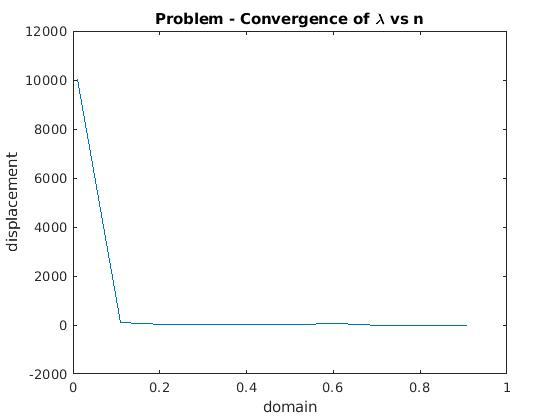
\includegraphics[width=\textwidth]{setTwo.jpg}
		\caption{0 - n - 1}
		\label{fig:setTwo.jpg}
	\end{subfigure}
	\begin{subfigure}[h!]{0.4\textwidth}
		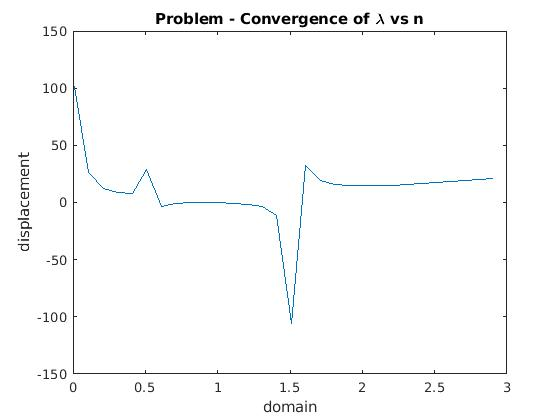
\includegraphics[width=\textwidth]{setThree.jpg}
		\caption{0 - n - 3}
		\label{fig:setThree.jpg}
	\end{subfigure}
	\begin{subfigure}[h!]{0.4\textwidth}
		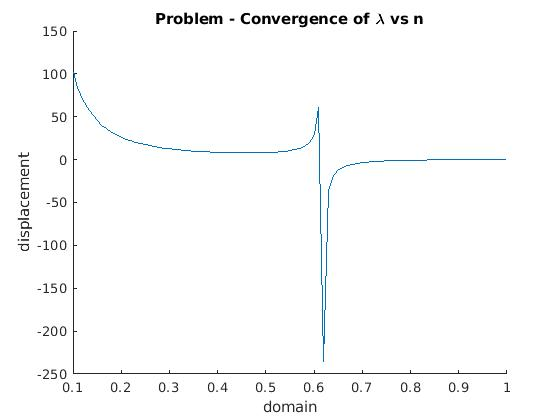
\includegraphics[width=\textwidth]{setFour.jpg}
		\caption{0.1 - n - 1}
		\label{fig:setFour.jpg}
	\end{subfigure}
	\begin{subfigure}[h!]{0.4\textwidth}
		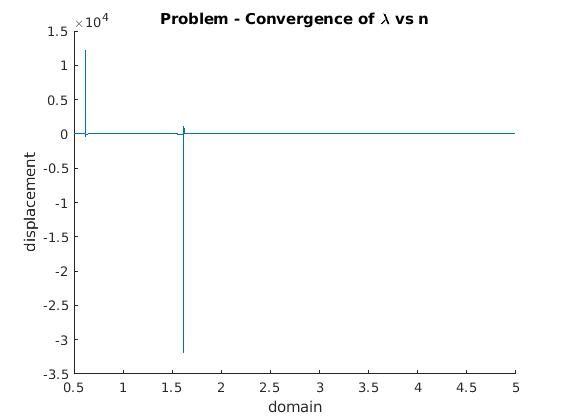
\includegraphics[width=\textwidth]{setSeven.jpg}
		\caption{0.5 - n - 5}
		\label{fig:setSeven.jpg}
	\end{subfigure}
	\caption\Large\textbf{Variation of $\lambda$ for varying ellipticity}
\end{figure}


%This is a bulleted list:
%
%\begin{itemize}
%\item Item 1
%\item Item 2
%\item \ldots and so on
%\end{itemize}
%
%%%-----------------------------------------
%%
%%\experiment{example}
%%
%%\lipsum[6]
%%
%%%-----------------------------------------
%%
%%\experiment{example2}
%%
%%\lipsum[7]
%%
%%%----------------------------------------------------------------------------------------
%%	FORMULAE AND MEDIA RECIPES
%%----------------------------------------------------------------------------------------
%
%\labday{} % We don't want a date here so we make the labday blank
%
%\begin{center}
%\HRule \\[0.4cm]
%{\huge \textbf{Formulae and Media Recipes}}\\[0.4cm] % Heading
%\HRule \\[1.5cm]
%\end{center}
%
%%----------------------------------------------------------------------------------------
%%	MEDIA RECIPES
%%----------------------------------------------------------------------------------------
%
%\newpage
%
%\huge \textbf{Media} \\ \\
%
%\normalsize \textbf{Media 1}\\
%\begin{table}[H]
%\begin{tabular}{l l l}
%\toprule
%\textbf{Compound} & \textbf{1L} & \textbf{0.5L}\\
%\toprule
%Compound 1 & 10g & 5g\\
%Compound 2 & 20g & 10g\\
%\bottomrule
%\end{tabular}
%\caption{Ingredients in Media 1.}
%\label{tab:med1}
%\end{table}
%
%%-----------------------------------------
%
%%\textbf{Media 2}\\ \\
%
%%Description
%
%%----------------------------------------------------------------------------------------
%%	FORMULAE
%%----------------------------------------------------------------------------------------
%
%\newpage
%
%\huge \textbf{Formulae} \\ \\
%
%\normalsize \textbf{Formula 1 - Pythagorean theorem}\\ \\
%$a^2 + b^2 = c^2$\\ \\
%
%%-----------------------------------------
%
%%\textbf{Formula X - Description}\\ \\
%
%%Formula
%
%%----------------------------------------------------------------------------------------

\end{document} 